\subsection{Virtualization}

A basic layered architecture of the Virtual Machines running application workloads is as below in [Fig. 10] based on the explanation from [3]

\begin{figure}[h!]
    \centering
    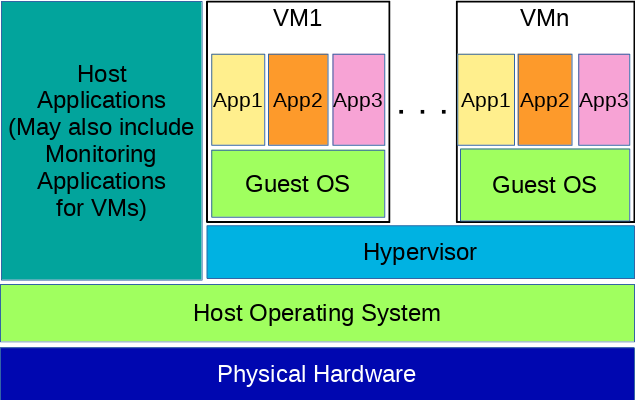
\includegraphics[width=0.5\textwidth]{vm_layers}
    \label{fig:figure9}
    \caption{Components of Virtualization}
\end{figure}

In traditional virtualization, also refered to as hardware virtualization, a hypervisor (eg: KVM) emulates the hardware into a guest and isolates it from other KVM instances. An Operating System can be installed and the KVM instance can then be used as an independent system for any application. The interaction between the application running on the Guest Operating system and the host operating system kernel is through the intermediate interface called the Hypercall. The hypervisor needs a virtual switch which it can connect to using tap interfaces to communicate with other Virtual Machines (KVM instances). Libraries such as Libvirt provide interfaces to interact with the KVM instances with ease.
